\documentclass{article}
\usepackage[english]{babel}
\usepackage[utf8]{inputenc}
\usepackage[T1]{fontenc}
\usepackage{graphicx}
\usepackage{caption}
\usepackage{subcaption}
\usepackage{float}
\usepackage{wrapfig}
\usepackage{setspace}
\usepackage{cite}
\usepackage{url}
\usepackage{color}
\definecolor{linkcol}{rgb}{0,0,0.4}
\definecolor{citecol}{rgb}{0.5,0,0}
\usepackage[pagebackref,hyperindex=true]{hyperref}
\hypersetup{colorlinks=true,linkcolor=linkcol,citecolor=citecol,urlcolor=linkcol}

\usepackage{amsmath}
\usepackage{amssymb}
\usepackage{amsfonts}
\usepackage{amsopn}
\usepackage{braket}
\usepackage{bbm}
\usepackage{dsfont}
\usepackage{kpfonts}
% \usepackage{mathabx}

\parindent=0cm


% Various new commands that ease typesetting math even further
% \newcommand{\assign}{\ensuremath{\coloneq}}
% \newcommand{\rassign}{\ensuremath{\eqcolon}}
\newcommand{\assign}{\ensuremath{:=}}
\newcommand{\rassign}{\ensuremath{=:}}

\newcommand{\of}[1]{\ensuremath{\left( #1 \right)}}
\newcommand{\ofs}[1]{\ensuremath{\left( #1 \right)}}

\newcommand{\norm}[1]{\ensuremath{\| #1 \|}}

\newcommand{\tmop}[1]{\ensuremath{\operatorname{#1}}}

\newcommand{\id}{\ensuremath{\mathds{1}}}
% \newcommand{\id}{\ensuremath{I}}


\newcommand{\conj}[1]{\ensuremath{\overline{#1}}}

\newcommand{\T}{\ensuremath{{}^{\textnormal{T}}}}
\newcommand{\herm}{\ensuremath{{}^{\textnormal{H}}}}

\newcommand{\ft}[1]{\ensuremath{\mathcal{F}\left(#1\right)}}
\newcommand{\ift}[1]{\ensuremath{\mathcal{F}^{-1}\left(#1\right)}}

\newcommand{\fft}[1]{\ensuremath{\mathtt{FFT}\left(#1\right)}}
\newcommand{\ifft}[1]{\ensuremath{\mathtt{IFFT}\left(#1\right)}}

\newcommand{\dotp}[2]{\ensuremath{\langle #1 , #2 \rangle}}

\newcommand{\bigO}[1]{\ensuremath{\mathcal{O}\left( #1 \right)}}

\newcommand{\mat}[1]{\ensuremath{\mathbf{#1}}}

% multi-indices
\newcommand{\mindex}[1]{\ensuremath{\underline{#1}}}

\newcommand{\laplace}{\ensuremath{\operatorname{\Delta}}}

% EOF

 
\usepackage[ruled]{algorithm2e}

% Configure Algorithm2e
\DontPrintSemicolon
\SetKwInOut{Input}{Input}
\SetKwInOut{Output}{Output}

\def\code#1{\texttt{#1}}
\def\classname#1{\textit{#1}}
\def\filename#1{\textit{#1}}

\newtheorem{definition}{Definition}

\begin{document}

\begin{titlepage}
	\begin{center}

		\hfill

		\vspace{2cm}

		{\huge \textsc{Time Propagation\\ of Quantum Wave Packets\\[10pt]}}
		{\Large \textsc{an efficient implementation in C++\\[10pt]}}

		\vspace{1cm}

		{\Large{Bachelor Thesis}}

		\vspace{1cm}

		{\emph{written by}} \\
		{
			Matthias Untergassmair
		}

		\vspace{1cm}

		{\emph{advised by}} \\
		{
			Raoul Bourquin
		}

		\vspace{1cm}

		{\emph{supervised by}} \\
		{
			Dr. Vasile Gr\u{a}dinaru\\
			Prof. Dr. Ralf Hiptmair
		}
		
		\vfill

		Seminar for Applied Mathematics\\
		ETH Zurich

		\vspace{.5cm}

		\emph{{Fall semester 2016}}

		\vspace{.5cm}

		
\includegraphics[width=0.5\linewidth]{figures/eth-logo.pdf}

	\end{center}

\end{titlepage}


\tableofcontents
\clearpage

\section{Introduction}
The topic of this thesis is the C++ reimplementation of the library WaveBlocksND
\cite{waveblocksnd}, which is written in Python.
This report describes the inner working of my C++ implementation
and explains the reasoning behind important software designs choices.
This report doesn't explain the theory behind Hagedorn wavepackets.
For an introduction to Hagedorn wavepackets, I refer to some earlier work
of George A. Hagedorn \cite{H_ladder_operators}.
The technical details of WaveBlocksND are explained
in the master thesis of Raoul Bourquin \cite{B_master_thesis}.

WaveBlocksND implements the time propagation of Hagedorn wavepackets.
The extent is too large for a bachelor thesis, therefore I focused on the
evaluation and gradient computation of Hagedorn wavepackets.
I made extensive use of Eigen \cite{eigenweb}, a C++ template library for linear algebra.

\section{Basis shape}

A \(D\)-dimensional basis shape \(\mathfrak{K}\)
is a set of \emph{unordered} D-dimensional integer-tuples, also
referred to as \emph{nodes}.  A shape is suitable for our needs, if it
satisfies the fundamental property

\begin{equation}
  \label{eq:basis_shape_fundamental_property}
  \mindex{k} \in \mathfrak{K} \Rightarrow \forall
  \mindex{k}-\mindex{e}^d \in \mathfrak{K} \;\forall d \in \{d \;|\;k_d \geq 1\}
\end{equation}

where \(\mindex{e}^d\) is the unit vector in direction \(d\).
That means, if an arbitrary node is part of the basis shape, then all nodes
in the backward cone are part of the shape too.

\subsection{Basis shape description}
In WaveBlocksND, implementing a shape is quite involved since you
not only have to describe which nodes lie in a shape (which is easy),
as well you have to provide node iterators in two flavours (which is hard).
In my implementation, the iterator part is a service provided by the
\emph{shape enumerator}. Thus, if you want to use a new shape type in your simulation,
all you have to do, is to provide an algebraic description, that describes
which nodes are part of the shape. The shape enumerator takes care of the rest.

This algebraic description consists of a set of surface functions and
a minimum bounding box.

\begin{definition}[Surface functions of basis shapes]
  The \(D\) surface functions of an arbitrary \(D\)-dimensional shape are defined by
  \begin{equation}
  s_{\alpha}(\mindex{n})=\max
    \left\{k_{\alpha} \mid \mindex{k} \in \mathfrak{K} \land
      k_d = n_d \; \forall d \neq \alpha
    \right\}
    \label{eq:basis_shape_surface_function}
  \end{equation}
\end{definition}

These functions are well-defined, because of the fundamental shape property
(\ref{eq:basis_shape_fundamental_property}).
This definition looks intricate, but once understood, defining shapes with it
is straightforward.

\begin{definition}[Minimum bounding box of basis shapes]
  The minimum bounding box describes the smallest
  box, within which all shape nodes lie.
  \begin{equation}
    L_{\alpha}=\max\left\{k_{\alpha} \mid \mindex{k} \in \mathfrak{K}\right\}
    \label{eq:basis_shape_bbox}
  \end{equation}
\end{definition}

\begin{figure}[H]
  \centering
  \begin{subfigure}[]{0.4\textwidth}
    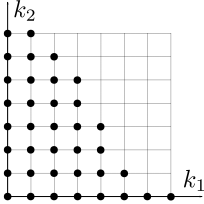
\includegraphics[width=1.0\textwidth]{shape_example}
    \label{fig:shape_example}
  \end{subfigure}
  ~
  \begin{subfigure}[]{0.5\textwidth}
    \begin{tabular}{|| c | c || c | c ||}
      \(\mindex{n}\) & \(s_1(\mindex{n})\) & \(\mindex{n}\) & \(s_2(\mindex{n})\) \\
      (?, 0) & 7 & (0, ?) & 7 \\
      (?, 1) & 5 & (1, ?) & 7 \\
      (?, 2) & 4 & (2, ?) & 6 \\
      (?, 3) & 4 & (3, ?) & 5 \\
      (?, 4) & 3 & (4, ?) & 3 \\
      (?, 5) & 3 & (5, ?) & 1 \\
      (?, 6) & 2 & (6, ?) & 0 \\
      (?, 7) & 1 & (7, ?) & 0 \\
      (?, 8) & \(-\infty\) & (8, ?) & \(-\infty\) \\
    \end{tabular}
  \end{subfigure}
  \caption{Surface description of an 2-dimensional basis shape.}
\end{figure}

\subsection{Common basis shapes}
\begin{definition}[Hypercubic basis shape]
  Given the limits \(\mindex{K} \in \mathbb{N}^D\), a hypercubic shape is defined by

  \begin{equation}
    \label{eq:hypercubic_shape}
    \mathfrak{K}(D,\mindex{K}) \coloneqq \left\{(k_1,\dots,k_D) \in \mathbb{N}_0^D \;|\; k_d < K_d \forall d\right\}
  \end{equation}
\end{definition}

We derive the surface functions by inserting (\ref{eq:hypercubic_shape}) into
equation
(\ref{eq:basis_shape_surface_function}):
\[
  s_{\alpha}(\mindex{n})=\max\left\{k_{\alpha} \mid (k_{\alpha}<K_{\alpha}) \;\land\;
    (n_d < K_d \;\forall d \neq \alpha)\right\}
\]

\begin{equation}
  s_{\alpha}(\mindex{n})=
  \begin{cases}
    K_{\alpha}-1 & n_d < K_d \;\forall d \neq \alpha \\
    -\infty & otherwise \\
  \end{cases}
\end{equation}

We retrieve the minimum bounding box by inserting (\ref{eq:hypercubic_shape}) into
equation
(\ref{eq:basis_shape_bbox}):

\[
L_{\alpha}=\max\left\{k_{\alpha} \mid k_{\alpha}<K_{\alpha}\right\}
\]

\begin{equation}
L_{\alpha}=K_{\alpha}-1
\end{equation}

\begin{definition}[Hyperbolic cut basis shape]
  Given the sparsity parameter \(S \geq 1\), a hyperbolic cut shape is defined by
  \begin{equation}
    \mathfrak{K}(D,S) \coloneqq \left\{(k_1,\dots,k_D) \in \mathbb{N}_0^D \;|\;\prod_{d=1}^D(k_d+1) \leq S\right\}
    \label{eq:hyperbolic_cut_shape}
  \end{equation}
\end{definition}

We derive the surface functions by inserting (\ref{eq:hyperbolic_cut_shape}) into
equation (\ref{eq:basis_shape_surface_function}):

\[
  s_{\alpha}(\mindex{n})=
  \max\left\{k_{\alpha} \mid (k_{\alpha}+1)\prod_{d \neq \alpha} (n_d+1) \leq S \right\} =
  \max\left\{k_{\alpha} \mid k_{\alpha}+1 \leq \frac{S}{\prod_{d \neq \alpha}(n_d+1)}\right\}
\]

\begin{equation}
s_{\alpha}(\mindex{n})=\frac{1}{\prod_{d \neq \alpha} (n_d+1)}-1
\end{equation}

We retrieve the minimum bounding box by inserting (\ref{eq:hyperbolic_cut_shape}) into
equation (\ref{eq:basis_shape_bbox}):

\[
  L_{\alpha}=\max\left\{k_{\alpha} \mid \prod_{d=1}^D(k_d+1) \leq S\right\} =
  \max\left\{k_{\alpha} \mid k_{\alpha}+1 \leq \frac{S}{\prod_{d \neq \alpha}(k_d+1)}\right\}
\]

\begin{equation}
L_{\alpha}=S-1
\end{equation}

\begin{definition}[Shape intersection]
  The intersection of the shapes \(\mathfrak{K}^{A}\) and \(\mathfrak{K}^{B}\) is defined by
  \begin{equation}
    \label{eq:basis_shape_intersection}
    \mathfrak{K}^{A \cap B}=\left\{\mindex{k} \;|\; \mindex{k} \in \mathfrak{K}^A \land
      \mindex{k} \in \mathfrak{K}^B
    \right\}
  \end{equation}
\end{definition}

Using equation (\ref{eq:basis_shape_surface_function}) and (\ref{eq:basis_shape_bbox})
we obtain the surface functions

\begin{equation}
  s_{\alpha}^{A \cap B}(\mindex{n}) = \min\{s_{\alpha}^A(\mindex{n}), s_{\alpha}^B(\mindex{n})\}
\end{equation}

and the minimum bounding box

\begin{equation}
  L_{\alpha}^{A \cap B} = \min\{L_{\alpha}^{A}, L_{\alpha}^{B}\}
\end{equation}

Remark: The \emph{limited hyperbolic cut shape} is an intersection of an
\emph{hypercubic shape} and a \emph{hyperbolic cut shape}.

\begin{definition}[Shape union]
  The union of the shapes \(\mathfrak{K}^{A}\) and \(\mathfrak{K}^{B}\) is defined by
  \begin{equation}
    \label{eq:basis_shape_union}
    \mathfrak{K}^{A \cup B}=\left\{\mindex{k} \;|\; \mindex{k} \in \mathfrak{K}^A \lor
      \mindex{k} \in \mathfrak{K}^B
    \right\}
  \end{equation}
\end{definition}

Using equation (\ref{eq:basis_shape_surface_function}) and (\ref{eq:basis_shape_bbox})
we obtain the surface functions

\begin{equation}
  s_{\alpha}^{A \cup B}(\mindex{n}) = \max\{s_{\alpha}^A(\mindex{n}), s_{\alpha}^B(\mindex{n})\}
\end{equation}

and the minimum bounding box

\begin{equation}
  L_{\alpha}^{A \cup B} = \max\{L_{\alpha}^{A}, L_{\alpha}^{B}\}
\end{equation}

\subsection{Basis shape slicing} \label{sec:basis_shape_slice}
Many algorithms, notably the evaluation of a Hagedorn wavepacket,
use recursive formulas of the form
\( \phi_{\mindex{k}} = f(\phi_{\mindex{k}-\mindex{e}^1}, \ldots,
\phi_{\mindex{k}-\mindex{e}^D}) \)
where \( \phi_{\mindex{k}} \)
is a value associated with the node \( \mindex{k} \) and
\( \mindex{e}^d \) is the unit vector in direction \( d \).
Thus, it is beneficial to organize a shape into slices.

\begin{definition}[Basis shape slice]
  \label{eq:basis_shape_slice}
  Basis shapes \(\mathfrak{K}\) are divided into disjoint slices \(\mathfrak{S}\)
  \begin{equation}
    \mathfrak{K}=\bigcup_{s=0}^{\infty} \mathfrak{S}^s
  \end{equation}

  The \( s \)-th
  slice \( \mathfrak{S}^s \) of a shape \( \mathfrak{K} \)
  contains all nodes \( \mindex{k} \in \mathfrak{K} \)
  that satisfy
  \begin{equation}
    \sum_{d=1}^{D} k_d = s
  \end{equation}
  Apparently, \(s\) is the Manhattan distance or $l_1$ norm to the origin.
\end{definition}

\begin{figure}[H]
  \centering
  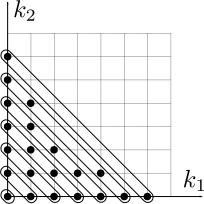
\includegraphics[]{shape_slicing}
  \caption{A basis shape and its slicing.}
\end{figure}


\subsection{Basis shape enumeration}
A basis shape description just tells, whether it contains a specific node.
But we need to associate coefficients \(c_{\mindex{k}}\)
and basis functions \(\phi_{\mindex{k}}\) with shape
nodes \(\mindex{k}\). We can use a hash table to map \(\mindex{k}\) to
\(c_{\mindex{k}}\), \(\phi_{\mindex{k}}\). But it is simpler to
enumerate all nodes in a shape. This means, if a multi-index \(\mindex{k}\)
maps to an ordinal \(i\), we find \(\phi_{\mindex{k}}\) at the position
\(i\) in the array  \(\{\phi\}\).
This way, we can keep coefficients and basis function values in an array,
ordered according to the shape enumeration.

\begin{definition}
  A shape enumeration is a bijective mapping that orders all nodes
  of \( \mathfrak{K} \)
  and assigns the \(i\)-th node the ordinal \(i\).
\end{definition}

Remark: Due to the close relationship of the enumeration to the shape,
the symbol \(\mathfrak{K}\) is used for both shape and
shape enumeration.

\subsubsection{Shape enumeration algorithm}

\begin{figure}[H]
  \centering
  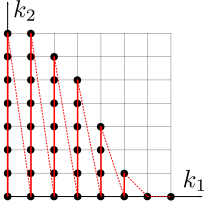
\includegraphics[]{shape_enumerator}
  \caption{Enumerator passage through a 2-dimensional basis shape}
  \label{fig:shape_enumerator}
\end{figure}

The enumerator takes a description of a basis shape and enumerates it in two passes.

In the first pass, knowing the surface functions \(s_{\alpha}\)
and the minimum bounding volume \(L_{\alpha}\) of a shape,
the enumerator iterates through all nodes inside the basis shape in lexicographical order.
Each node is subsequently appended to the proper slice (see section (\ref{sec:basis_shape_slice})).
In the second pass, the enumerator determines the offset of each slice.
The offset is the number of all nodes in previous slices. Equivalently, it is the
ordinal of the first node of the slice (if assuming zero-based arrays).

\begin{algorithm}[H]
  \emph{Enumerate all nodes in lexicographical order}\;
  \For{\(k_1 \leftarrow 0\) \KwTo \(s_1((0,0,0))\)}{
    \For{\(k_2 \leftarrow 0\) \KwTo \(s_2((k_1,0,0))\)}{
      \For{\(k_3 \leftarrow 0\) \KwTo \(s_3((k_1,k_2,0))\)}{
        \emph{Append lattice node to its slice} \;
        \(\mathfrak{S}_{k_1+k_2+k_3} \leftarrow \mathfrak{S}_{k_1+k_2+k_3} \cup \, (k_1,k_2,k_3) \)
      }
    }
  }
  \caption{Enumerator passage through a 3-dimensional basis shape.}
  \label{fig:enumerator_pass_3d}
\end{algorithm}

Remark: This algorithm is recursive (one loop for each dimension).
The real implementation however is iterative.

\subsubsection{Data structure}

The enumerator data structure is as follows

\begin{verbatim}
template<dim_t D, class MultiIndex>
struct ShapeEnum {
    std::vector< ShapeSlice<D,MultiIndex> > slices;
};
\end{verbatim}

\begin{verbatim}
template<dim_t D, class MultiIndex>
struct ShapeSlice {
    std::size_t offset;
    std::vector< MultiIndex > table;
};
\end{verbatim}

The class \classname{ShapeEnum} representing \(\mathfrak{K}\) contains a list
of all non-empty shape slices. The class \classname{ShapeSlice}
\(\mathfrak{S}^s\) contains an array of all nodes \(\mindex{k} \in \mathfrak{S}^s\).

All multi-indices of a slice are lexicographically ordered.
The lexicographical order begins on the first index, continues to the second index and so forth.
\begin{equation}
  \label{eq:lexicographical_order}
  a_1a_2\dots a_D <_{lex}b_1b_2\dots b_D \iff
  \begin{cases}
    (a_1 < b_1) \lor (a_1 = b_1 \land a_2\dots a_D <_{lex} b_2\dots b_D) & D > 1 \\
    (a_1 < b_1) & D = 1 \\
  \end{cases}
\end{equation}

\subsubsection{Queries}
The two main operations of a shape enumeration are:
\begin{description}
\item[Retrieve the multi-index \(\mindex{k}\) associated with a given ordinal \(i\)]\mbox{}
  \par
  All multi-indices of a shape are stored in an array.
  Thus, we simply return the \(i\)-th multi-index.
  \par
  Run-time complexity: \(\mathcal{O}(1)\)
\item[Find the ordinal \(i\) of a given multi-index \(\mindex{k}\)]\mbox{}
  \par
  First we have to determine, to which slice \(\mathfrak{S}^s\) the multi-index \(\mindex{k}\) belongs by
  computing \(s = \sum k_d \).\par
  All nodes inside a slice are ordered lexicographically. Therefore
  we determine the position of the node \(\mindex{k}\) inside the slice using \textbf{binary search}.
  The final ordinal is the position of \(\mindex{k}\) inside its slice plus
  the number of nodes in all previous slices.
  \par
  Run-time complexity: \(\mathcal{O}(\log{}S)\), where \(S\) is the size of the slice.

\end{description}

\subsubsection{Finding backward neighbours}
A common task is looking up all backward neighbours \(\{\mindex{k}-\mindex{e}^1,\ldots,\mindex{k}-\mindex{e}^D\}\)
of a node \(\mindex{k}\). This task can be slightly optimized: First, all neighbours live inside the same slice.
Secondly, they are ordered i.e. \((\mindex{k}-\mindex{e}^d)\) is stored before \((\mindex{k}-\mindex{e}^{d+1})\).
Thirdly, due to how lexicographical order works, the distance between \((\mindex{k}-\mindex{e}^{d-1})\) and \((\mindex{k}-\mindex{e}^d)\)
is usually much larger than the distance between \((\mindex{k}-\mindex{e}^d)\) and \((\mindex{k}-\mindex{e}^{d+1})\).
The following algorithm takes advantage of this alignment by defining a search range \([a;b]\),
which is the whole slice at the beginning.
After each determined ordinal, the algorithm subsequently reduces the search range
of the remaining nodes.

\begin{algorithm}[H]
  \caption{Algorithm to find ordinals of backward neighbours}
  \Input{Node \(\mindex{k}\).}
  \Input{Slice that contains the backward neighbours \(\mathfrak{S}\).}
  \Output{Ordinals of backward neighbours \(\{i^1,\ldots,i^D\}\).}
  \(a \leftarrow 1\)\;
  \(b \leftarrow size(\mathfrak{S})\)\;
  \(i^D \leftarrow find(\mindex{k}-\mindex{e}^D) \in \mathfrak{S}[a;b]\)\;
  \(b \leftarrow i^D\)\;
  \For{\(d \leftarrow 1\) \KwTo \(D-1\)}{
    \(i^d \leftarrow find(\mindex{k}-\mindex{e}^d) \in \mathfrak{S}[a;b]\)\;
    \(a \leftarrow i^d\)\;
  }
\end{algorithm}

\subsubsection{Multi-index representation}
The size of a multi-index has a big influence to lookup times and
overall simulation time. Therefore the user can choose at compile-time an appropriate
type to represent multi-indices. I provide the class \classname{TinyMultiIndex}
that packs the whole multi-index into 64 bits.
Multi-indices of accomplishable simulations should fit into 64 bits.
Otherwise you can define a new multi-index type. A custom implementation
must possess the same semantics as \code{std::array<int,D>}.
Furthermore it has to specialize \code{std::less} that performs lexicographical index comparison
beginning on the first index.
And it has to specialize \code{std::equal\_to} and \code{std::hash} to
enable use of multi-indices as hash table keys.

\subsubsection{Alternative data structures}
I tried a hash table (\code{std::unordered\_set}) to map multi-indices to ordinals.
To represent multi-indices, I used the tiny (64 bits) representation.
These 64 bits can be used unmodified as a hash value.
But queries proved to be 2-3 times slower compared to binary search,
despite of \(\mathcal{O}(1)\) compared to \(\mathcal{O}(\log{}n)\) lookup time.
\par
Hash Tables are good when querying random keys. But an algorithm working
with basis shapes does \emph{not} access random nodes.
Such algorithms typically access neighbours of previously accessed nodes.
The problem is, that hash tables
map neighbour nodes to seemingly random locations in memory,
while an sorted array keeps neighbours together. Thus, a hash table triggers
a lot more cache misses, than binary search on an sorted array.

\subsection{Basis shape extension}

We need basis shape extensions to compute wavepacket gradients.

\begin{definition}[Extended basis shape]
  Given a basis shape \( \mathfrak{K} \),
  the shape extension \( \mathfrak{K}_{ext} \) is defined by
  \begin{equation}
    \mathfrak{K}_{ext} \coloneqq \mathfrak{K} \cup
    \left\{\mindex{k}' \mid \mindex{k}' = \mindex{k} + \mindex{e}^d
      \forall \mindex{k} \in \mathfrak{K} \forall d\right\}
  \end{equation}
  where \( \mindex{e}^d \) is the unit vector in direction \( d \).
\end{definition}

\begin{figure}[H]
  \begin{center}
    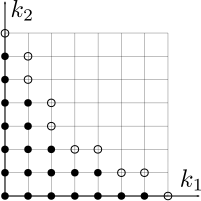
\includegraphics[width=0.5\linewidth]{shape_extension}
  \end{center}
  \caption{Basis shape (filled bullets) and its extension (empty
    bullets).}
\end{figure}

While is possible to define surface functions of the extension,
creating an extended shape this way is impractical.
The basis shape extension is needed, when
we have to compute the gradient of a wavepacket. At this stage,
the wavepacket's basis shape is in its enumerated form,
basically just an array of multi-indices. The original shape description is not available.
Therefore, we somehow have to create the extension out of the enumerated form.
\par
This task turns out rather straight-forward. We take one slice \(\mathfrak{S}^s\) of
the input basis shape, clone it and
shift it one unit to direction \(d\) by incrementing the \(d\)-th index of every multi-index.
We create one clone for each direction. Then we merge these \(D\) clones and get the
slice \(\mathfrak{S}_{ext}^{s+1}\) of the extended shape.
Notice that nodes inside a clone are already lexicographically ordered.
Thus, during the merge operation, we just have to interleave the clones in such a way that
lexicographical order is kept and duplicates get eliminated.
Using a divide and conquer approach, the total algorithmic complexity is
\(\mathcal{O}(D\log{}D \cdot N)\), where \(D\) is the wavepacket dimensionality and \(N\)
is the number of basis shape nodes.

\begin{algorithm}[H]
  \caption{Create extended shape of an already enumerated basis shape.}
  \Input{Enumerated basis shape (slices) \(\mathfrak{K}=\bigcup_s\mathfrak{S}^s\)}
  \Output{Basis shape extension (slices) \(\mathfrak{K}_{ext}=\bigcup_s\mathfrak{S}_{ext}^s\)}
  \(\mathfrak{S}_{ext}^0 \leftarrow \mindex{0}\)\;
  \ForEach{\(\mathfrak{S}^s \in \mathfrak{K}\)}{
    \For{\(d \leftarrow 1\) \KwTo \(D\)}{
      \(\mathfrak{S}_{ext}^{s+1} \leftarrow \mathfrak{S}_{ext}^{s+1} \cup
      \left\{\mindex{k}+\mindex{e}^d \;\forall \mindex{k} \in \mathfrak{S}^s\right\}\)\;
    }
  }
\end{algorithm}

\section{Hagedorn wavepackets}
\subsection{Scalar wavepackets}
A \(D\)-dimensional scalar Hagedorn wavepacket is a linear combination of basis functions \(\phi_{\mindex{k}}\)
with coefficients \(c_{\mindex{k}}\)

\begin{equation}
  \label{eq:scalar_hawp_inf}
  \ket{\Phi} \coloneqq \Phi[\Pi](\vec{x}) = \exp{\left(\frac{iS}{\varepsilon^2}\right)}
  \sum_{\mindex{k} \in \mathbb{N}^D} c_{\mindex{k}}\phi_{\mindex{k}}[\Pi](\vec{x})
\end{equation}

where \(\varepsilon\) is the semi-classical scaling parameter.\par
Notice that \(\mindex{k}\) is a \emph{multi-index}. It is a tuple that
contains \(D\) integers called indices.
The basis functions \(\phi_{\mindex{k}}\) depend on the
Hagedorn parameter set \(\Pi\). It is a tuple
\[
  \Pi \coloneqq \left(\vec{q},\vec{p},\mat{Q},\mat{P},S\right)
\]
containing the vectors \( \vec{q},\vec{p} \in \mathbb{R}^D \) and
complex matrices \( \mat{Q},\mat{P} \in \mathbb{C}^{D \times D} \). \(S\in \mathbb{C}\) is
the global phase factor.

Equation (\ref{eq:scalar_hawp_inf}) contains infinitely many basis functions.
To compute the wave\-packet we have to truncate the set of all basis functions to
a finite set \(\mathfrak{K} \subset \mathbb{N}^D\) called \emph{basis shape}.
The wavepacket equation becomes

\[
  \Phi[\Pi](\vec{x}) \approx \exp{\left(\frac{iS}{\varepsilon^2}\right)}
  \sum_{\mindex{k} \in \mathfrak{K}}c_{\mindex{k}}\phi_{\mindex{k}}[\Pi](\vec{x})
\]

To specify a Hagedorn wavepacket I often use the tuple notation

\[
  \Phi \coloneqq  \left(\varepsilon,\Pi,\mathfrak{K},c\right)
\]

\subsection{Vectorial wavepackets}
Vectorial Hagedorn wavepackets \(\Psi\) consist of multiple components \(\Phi_i\)
\[
  \Psi(\vec{x}) \coloneqq
  \begin{pmatrix}
    \Phi_1(\vec{x}) \\
    \Phi_2(\vec{x}) \\
    \vdots \\
    \Phi_N(\vec{x}) \\
  \end{pmatrix}
\]
The components \(\Phi_i\) itself are plain scalar wavepackets.
They have the scaling parameter \(\varepsilon\) in common, but
the Hagedorn parameter set and the basis shape may differ depending on
the concrete type. \\
Common vectorial wavepacket types are:
\begin{description}
\item[Inhomogeneous wavepacket]
  The inhomogeneous wavepacket is the most general case, as its components only share
  the scaling parameter \(\varepsilon\).
  \[
    \Phi_i \coloneqq  (\varepsilon, \Pi_i, \mathfrak{K}_i, c_i) \] \[
    \Psi \coloneqq  \left(\varepsilon,
    \begin{pmatrix}
      (\Pi_1, \mathfrak{K}_1, c_1) \\
      \vdots \\
      (\Pi_N, \mathfrak{K}_N, c_N) \\
    \end{pmatrix}\right)
  \]
\item[Homogeneous wavepackets]
  A homogeneous wavepacket is a special case of the inhomogeneous wavepacket.
  All components share the same Hagedorn parameter set \(\Pi\).
  \[
    \Phi_i \coloneqq  (\varepsilon, \Pi, \mathfrak{K}_i, c_i) \] \[
    \Psi \coloneqq  \left(\varepsilon, \Pi,
    \begin{pmatrix}
      (\mathfrak{K}_1, c_1) \\
      \vdots \\
      (\mathfrak{K}_N, c_N) \\
    \end{pmatrix}\right)
  \]
\item[Gradient]
  The gradient of a scalar Hagedorn wavepacket is a vectorial Hagedorn
  wavepacket. All components share the same Hagedorn parameter set and the
  same basis shape, which is an extension of the original wavepacket's basis shape.
  \[
    -i\varepsilon^2\frac{\partial \Phi}{\partial x_n} \coloneqq  (\varepsilon, \Pi, \mathfrak{K}_{ext}, c'_n) \] \[
    -i\varepsilon^2\nabla \Phi \coloneqq  \left(\varepsilon, \Pi, \mathfrak{K}_{ext},
    \begin{pmatrix}
      (c'_1) \\
      \vdots \\
      (c'_D) \\
    \end{pmatrix}\right)
  \]
\end{description}

\subsection{Class diagram}

\begin{figure}[H]
  \centering
  \includegraphics[width=1.0\textwidth]{hawp_inheritance}
  \caption{Wavepacket classes and the inheritance hierarchy.}
  \label{fig:hawp_inheritance}
\end{figure}

\subsubsection{Scalar wavepacket classes}

The superclass of all (scalar) Hagedorn wavepackets is \textbf{AbstractScalarHaWpBasis}.
It provides read-only access to \(\varepsilon\), \(\Pi\) and \(\mathfrak{K}\)
through its abstract virtual member functions \emph{eps()}, \emph{parameters()} and \emph{shape()}
respectively. It does not provide access to the coefficients \(\{c_k\}\), because coefficients
are not necessary to evaluate the basis functions \(\{\phi_k(\vec{x})\}\) on the grid nodes \(\vec{x}\),
which is implemented by the member function \textbf{evaluate\_basis(grid)}.
This function is not virtual, because it is a service provided by this base class.
All classes that inherit AbstractScalarHaWpBasis and thus provide access to \(\varepsilon\),
\(\Pi\) and \(\mathfrak{K}\) automatically gain the ability to evaluate their basis functions.

This superclass further implements the function \textbf{extended\-\_shape()},
which returns the basis shape extension \(\mathfrak{K}_{ext}\)
of the current basis shape \(\mathfrak{K}\). It is used for the gradient computation.
Creating a basis shape extension is expensive, therefore \(\mathfrak{K}_{ext}\) is cached.

The abstract class \textbf{AbstractScalarHaWp} extends the \classname{AbstractScalarHaWpBasis}.
It provides read-only access to the coefficients \(\{c_k\}\) through its virtual member function
\emph{coefficients()}. Thus it is able to evaluate itself \(\Phi(\vec{x})\) on the grid nodes \(\vec{x}\),
which is implemented by the member function \textbf{evaluate(grid)}.

\subsubsection{Vectorial wavepacket classes}
Vectorial wavepacket classes are implemented as a composition of scalar wave\-packets.
Shared aspects are stored in the composition class while different aspects are
stored in the component class.
Component classes inherit the features of the abstract scalar wavepacket class.
Therefore they have to implement access to the parameters \(\varepsilon\), \(\Pi\), \(\mathfrak{K}\)
and \(\{c_k\}\).
If a parameter is not stored inside the component class itself, but in the composition class,
the component class refers to the parameter stored inside the composition class.

Vectorial wavepacket classes provide a member function to evaluate itself, \(\Psi(\vec{x})\).
The return type is a vector, instead of a scalar value.
This function not only simplifies evaluation, it can considerably improve performance.
It exploits that components of homogeneous wavepackets share most basis
functions.\footnote{See section (\ref{sec:vector_hawp_eval}).}

\subsubsection{Rationale}

\textbf{Abstract superclasses don't provide writable access to parameters.}\par
Editing parameters of a superclass may have side-effects, you have no control over.
Some subclasses, like homogeneous wavepackets, share parameters across its components, while
others don't, like inhomogeneous wavepacket. It's not known at compile-time, what a
parameter change will cause. It may unintendedly change the parameters of many wavepackets.

However, concrete subclasses like ScalarHaWp, HomogeneousHaWp provide writable
access to its parameters. This is safe, because you know the concrete wavepacket type at compile-time.
Thus the behaviour is specified.
\par\bigskip
\textbf{Scalar and vectorial wavepackets don't have a common superclass.}\par
In WaveBlocksND, scalar and vectorial wavepackets actually have a common superclass.
It proved to be a bad design choice.
The problem is, that the evaluation function yields results
with different shape ranks, depending on the actual wavepacket type. It may
return a scalar, vector or even a matrix!
In python, this behaviour is halfway manageable, thanks to python's highly flexible type system
and numpy's broadcasting operations.
However, dealing with such behaviour is very hard in C++.
Therefore I decided, that scalar and vectorial wavepacket don't have a common superclass.
\par\bigskip
\textbf{There is no dedicated class to represent a gradient of a vectorial wavepacket.}\par
Applying the gradient operator to a vectorial wavepacket is trivial: Just apply it
to its components.
\[-i\varepsilon^2\nabla \Psi \equiv
\begin{pmatrix}
  -i\varepsilon^2\nabla \Phi_1 \\
  \vdots \\
  -i\varepsilon^2\nabla \Phi_N \\
\end{pmatrix}
\]
It is an overkill to introduce a new class, just to replace a loop.
Furthermore, storing all coefficients of \(-i\varepsilon^2\nabla\Psi\)
occupies \(\mathcal{O}(D \cdot N \cdot M)\) space.
Using a basis shape of a realistic size \(M=1'000'000\), and wavepacket
dimensionality \(D=10\), one can easily run out of memory.


\subsection{Basis evaluation}

All basis function values are evaluated recursively. Once we have the basis function
value at an anchor node \(\mindex{k}\) and the basis functions values on all
backward neighbours \(\mindex{k}-\mindex{e}^d\), we can compute all
forward neighbours by

\begin{equation}
  \begin{pmatrix}
    \phi_{\mindex{k}+\mindex{e}^1} \\
    \vdots \\
    \phi_{\mindex{k}+\mindex{e}^D}
  \end{pmatrix}
  = \left(
    \sqrt{\frac{2}{\varepsilon^2}} \mat{Q}^\mathrm{-1} (\vec{x}-\vec{q}) \phi_{\mindex{k}}
    - \mat{Q}^\mathrm{H} \mat{Q}^\mathrm{-T}
    \begin{pmatrix}
      \sqrt{k_1} \phi_{\mindex{k}-\mindex{e}^1} \\
      \vdots \\
      \sqrt{k_D} \phi_{\mindex{k}-\mindex{e}^D}
    \end{pmatrix}
  \right)
  \oslash
  \begin{pmatrix}
    \sqrt{k_1+1}\\
    \vdots \\
    \sqrt{k_D+1}
  \end{pmatrix}
\end{equation}

where the operator \(\oslash\) denotes a component-wise division.

\begin{figure}[H]
  \centering
  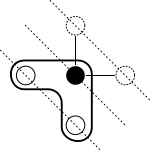
\includegraphics[]{basis_eval_stencil}
  \caption{Stencil of a 2-dimensional wavepacket}
\end{figure}

The root basis function \(\phi_{\mindex{0}}\) is evaluated by

\begin{equation}
  \label{eq:phi0_Dd}
  \phi_{\mindex{0}}[\Pi]\left(\vec{x}\right)
  \coloneqq
  (\pi\varepsilon^2)^{-\frac{D}{4}} (\det\mat{Q})^{-\frac{1}{2}}
  \exp \left( \frac{i}{2\varepsilon^2}
    \dotp{(\vec{x}-\vec{q})}{\mat{P}\mat{Q}^\mathrm{-1}(\vec{x}-\vec{q})}
    + \frac{i}{\varepsilon^2} \dotp{\vec{p}}{(\vec{x}-\vec{q})}
  \right)
\end{equation}

Basis functions with some negative indices are zero.

\subsubsection{Implementation}
There are two possibilities to implement this recursion scheme:
\begin{description}
\item[Scatter Type Strategy] We maintain a queue of anchor nodes whose
  basis functions already have been evaluated.
  We subsequently remove one feasible(!) entry \(\phi_{\mindex{k}}\) of this queue,
  evaluate the basis functions of all forward
  neighbours \(\phi_{\mindex{k}+\mindex{e}^d}\) and put these nodes back into the
  queue. To avoid multiple evaluation of basis functions, we
  have to check, whether a forward neighbour already has been computed,
  using a set. Therefore the scatter type strategy is very bad suited
  for multi-threading since threads need to synchronize access to this
  set.
\item[Gather Type Strategy] We maintain a queue of not yet evaluated
  forward neighbours \(\phi_{\mindex{k}+\mindex{e}^d}\). Entries of this queue can be evaluated
  since there exists a suitable\footnote{\(\phi_{\mindex{k}}\) and all \(\phi_{\mindex{k}-\mindex{e}^d}\)'s
  have been evaluated.}
  anchor node \(\phi_{\mindex{k}}\) we can apply the stencil on.
  We subsequently remove one entry of the queue and evaluate its basis function.
  Then we check, whether \emph{all} backward neighbours of the child
  node \(\phi_{\mindex{k}+\mindex{e}^d}\) are computed. If this is the case, we put all forward neighbours
  of \(\phi_{\mindex{k}+\mindex{e}^d}\) into the queue.
\end{description}

A straight-forward implementation has at least one of the following
difficulties, that require complex data structures, such as dictionaries
or would require excessive thread synchronisation.
\begin{description}
\item[A] We need to ensure that an already computed node is a valid
  anchor node (all backward neighbours has been computed too) so that
  we can compute its forward neighbours.
\item[B] We need to avoid multiple evaluation of the same node.
\end{description}

My rather simple solution is to split the basis shape into slices.  The
\(s\)-th slice contains all nodes \(\mindex{k}\) that fulfil
\( \sum_{d=1}^{D} k_d = s \).

\begin{figure}[H]
  \centering
  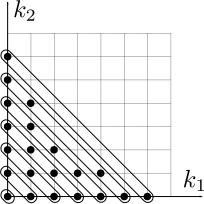
\includegraphics{shape_slicing}
  \caption{Slicing of a 2-dimensional basis shape.}
\end{figure}

Using an adequate\footnote{Fundamental property of a basis shape; see equation
  (\ref{eq:basis_shape_fundamental_property}).} shape,
the recursion scheme implies that if we had computed all basis
functions of the parent slice \( \mathfrak{S}^{s-1} \) and of the current
slice \( \mathfrak{S}^{s} \), then we can compute all basis functions of
the child slice \( \mathfrak{S}^{s+1} \) without having difficulty
\textbf{A}. Furthermore, if we use the gather type strategy where we
iterate through the child slice and compute its basis functions, we
automatically avoid difficulty \textbf{B}.

My solution has two compelling advantages:
\begin{description}
\item[Simple data structures] We can store the values of basis functions in
  an array. We need a \emph{shape enumeration}
  that maps shape nodes to ordinals, used as array offsets.
\item[Easy parallelisation] Parallelise the wavepacket evaluation is simple:
  Put an OpenMP pragma to the loop, that runs over the child slice.
  All previous slices have been completely computed,
  therefore the only synchronisation mechanism
  needed is a barrier at the end of the slice.
\end{description}

\begin{algorithm}[H]
  \Input{Number of slices \(S\)}
  \Input{Shape enumeration (slices)
    \(\mathfrak{K} = \left(\mathfrak{S}^0, \ldots,
      \mathfrak{S}^{S-1}\right)\)}
  \Output{Evaluated basis functions (slices) \(\phi \coloneqq  \left(\phi^0, \phi^1, \ldots, \phi^{S-1}\right)\)}
  \emph{Compute ground state}\;
  \(\phi^0 \gets \left\{ \phi_{\mindex{0}}[\Pi](\vec{x}) \right\} \)\;
  \emph{Loop over all slices}\;
  \ForEach{\(s \gets 0\) \KwTo \(S-2\)}{
    \emph{Loop over all
      nodes of next slice}\;
    \For{\(\mindex{k}^{s+1} \in \mathfrak{S}^{s+1}\)}{ \emph{Find
        suitable anchor node (in anchor slice \(\mathfrak{S}^s\))}\;
      \(\alpha \gets \varnothing \)\\
      \For{\(d \in \{1,\ldots,D\}\)}{
        \If{\(k^{s+1}_{d} > 0\)}{
          \(\alpha \gets d\)\;
        }
      }
      \emph{Here is our anchor node \(\mindex{k}^{s}\)}\;
      \(\mindex{k}^{s} \gets \mindex{k}^{s+1} - \mindex{e}^\alpha\)\;

      \emph{Compute contribution of anchor node}\;
      \(m \gets
      \frac{\sqrt{2}}{\varepsilon}\left(\mat{Q}^\mathrm{-1}(\vec{x}-\vec{q})\right)_\alpha\phi^{s}_{\mindex{k}^s}\)

      \emph{Compute contribution of anchor node's backward
        neighbours}\; \(b \gets 0\)\;
      \For{\(d \in \{1,\ldots,D\}\)}{
        \If{\(k^{s}_{d} > 0\)}{
          \(b \gets b + \sqrt{k^{s}_d}
          \left(\mat{Q}^{\mathrm{H}}\mat{Q}^{\mathrm{-T}}\right)_{\alpha
            d} \phi^{s-1}_{\mindex{k}^{s}-\mindex{e}^d}\)\; } }

      \emph{Compute basis function at \(\mindex{k}^{s+1}\)}\;
      \(\phi^{s+1}_{\mindex{k}^{s+1}} \gets
      \frac{1}{\sqrt{k^{s}_\alpha+1}}(m-b) \)
    }
  }
  \caption{Recursive basis evaluation of hagedorn wavepacket}
\end{algorithm}

\subsubsection{Algorithmic complexity} \label{sec:hawp_eval_runtime_complexity}
Evaluating \(D\)-dimensional wavepackets involves evaluating \(N\) basis functions.
To evaluate a basis function we have to lookup the ordinals of \(D\)
backward neighbours which costs \(\mathcal{O}(D \log{}S)\) because we use binary search.
\(S\) is the size of the largest slice. A shape has at least \(\mathcal{O}(D\log{}N)\)
slices (hypercubic shape). Therefore
\[
  \mathcal{O}(S)=\mathcal{O}(\frac{N}{D\log{}N}) \approx \mathcal{O}(N)
\]
Gathering values of previous basis functions \(\phi_{\mindex{k}-\mindex{e}^d}\) and computing \(\phi_{\mindex{k}}\)
has complexity \(\mathcal{O}(D)\).
Thus evaluating all basis functions has complexity
\[
  N \cdot \left(\mathcal{O}(D\log{}S) + \mathcal{O}(D)\right) =
  \mathcal{O}(ND\log{}S) \approx
  \mathcal{O}(N\log{}^2 N)
\]
when assuming \(D \approx \log{}N\).
Computing the dot-product \(\sum c_{\mindex{k}}\phi_{\mindex{k}}\) costs just \(\mathcal{O}(N)\)
thus the final \emph{asymptotic} complexity is
\begin{equation}
  \label{eq:hawp_eval_complexity}
  \mathcal{O}(N\log{}^2N)
\end{equation}

\subsubsection{Evaluating on multiple quadrature points at once}

To evaluate the basis function \(\phi_{\mindex{k}}\), we need all backward neighbours
\(\phi_{\mindex{k}-\mindex{e}^d}\).
Unfortunately the program spends much time on looking up the ordinals of these
backward neighbours. To improve the ratio of lookup time versus computation time,
I've implemented the possibility to evaluate the basis functions \(\phi_{\mindex{k}}\)
on multiple grid nodes at once. The number of grid nodes is a template parameter.

Figure (\ref{fig:hawp_eval_multiqp}) shows the effect of one
evaluation with \(N\) grid nodes compared to \(N\) evaluations with one
grid node each. It shows that the multi-node evaluation of a \(10\)-dimensional
wavepacket is on average up to \(3\) times faster than when using single-node evaluations.
The speedup is relatively independent on the dimensionality.
Deviations are caused by compiler optimizations and inner working of the Eigen library.

Notice, that you won't evaluate a wavepacket on let's say \(100'000\) quadrature points at once.
You will split these \(100'000\) quadrature points into chunks, each containing for example \(5\) nodes.
Then you evaluate the wavepacket on every chunk.
Compared to Python, in C++, there is no performance advantage in passing large
number of nodes to the evaluation function.
Far from it, you eventually run out of memory! Remember, that the evaluation function allocates memory for
\(\mathcal{O}(3SN)\) basis functions, where \(S\) is the size of the largest slice
and \(N\) is the number of grid nodes.

\begin{figure}[H]
  \centering
  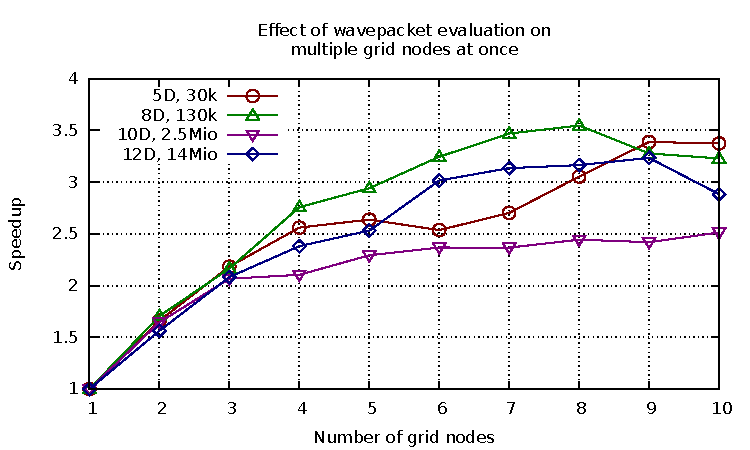
\includegraphics[width=1.0\textwidth]{plots/hawp_eval_multiqp}
  \caption{
    Effect of wavepacket evaluation on multiple quadrature points at once.
    The speedup is the cumulative run-time of single-node evaluations divided by
    the run-time of the multi-node-evaluation.
  }
  \label{fig:hawp_eval_multiqp}
\end{figure}

\subsection{Optimized evaluation of vectorial wavepackets} \label{sec:vector_hawp_eval}
The naive approach to evaluate vectorial wavepackets, is to separately
evaluate each component. For inhomogeneous wavepackets there is
no better way.
However components of homogeneous wavepackets share the same Hagedorn parameter set \(\Pi\)
and therefore share some basis functions. How many, depends on how large the overlap of
the basis shapes is. Basis shapes of components typically are very similar, therefore
the benefit of an algorithm, that exploits shape overlaps, can be considerable.

One way to achieve this, is to compute the union of the
basis shapes of all components:
\[
\mathfrak{K}^{\cup} \coloneqq  \mathfrak{K}^1 \cup \mathfrak{K}^2 \cup \dots \cup \mathfrak{K}^N
\]

Then we compute the basis functions governed by the basis shape union:
\[
\left\{\phi_{\mindex{k}} \;|\;\mindex{k} \in \mathfrak{K}^{\cup}\right\}
\]

Finally, for each wavepacket component \(\Phi_n\),
we compute the dot product of its coefficients \(c_{n,\mindex{k}}\)
with the subset \(\left\{\phi_{\mindex{k}}\;|\; \mindex{k} \in \mathfrak{K}^n\right\}\):

\[
\Phi_n(\vec{x})=\sum_{\mindex{k} \in \mathfrak{K}^n} c_{n,\mindex{k}} \phi_{\mindex{k}}(\vec{x})
\]

Remark: My implementation does the above computation slice by slice to save memory;
the same way as for a scalar wavepacket.

To quantify the improvement, I benchmarked the above algorithm on a homogeneous wavepacket with
varying number of components. All components have the same basis shape which is
the best case for the algorithm (since in this case, shapes completely overlap).
The 10-dimensional basis shape contains one million nodes.
The results (see figure \ref{fig:hawp_homogen_evaluation_speedup}) show that the
optimized algorithm can be six times faster than a naive loop over all
wavepacket components.

\begin{figure}[H]
  \centering
  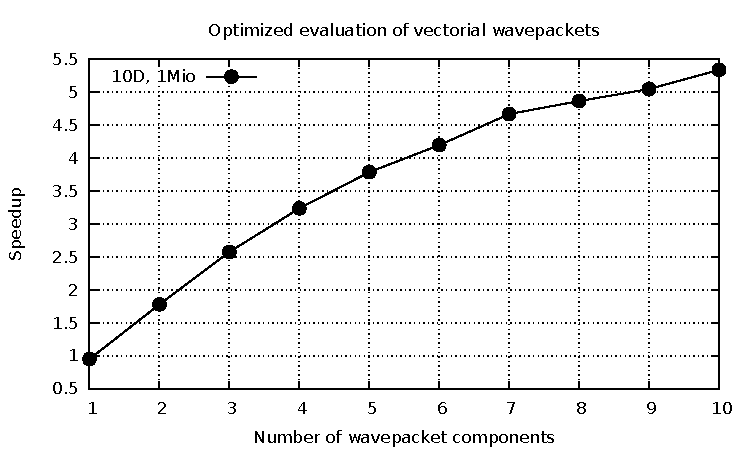
\includegraphics[width=1.0\textwidth]{plots/hawp_eval_homogen_speedup}
  \caption{
    Achievable speedup compared to naive evaluation of a vectorial wavepacket.
    The speedup is the run-time of the naive evaluation divided by the run-time of
    the optimized evaluation.
  }
  \label{fig:hawp_homogen_evaluation_speedup}
\end{figure}

There is an upper bound to the achievable speedup, as though the algorithm
avoids multiple evaluation of the same basis functions, it doesn't reduce
time spent on computing the dot products for each component.
Thus when increasing the number of wavepacket components, computing the dot-product becomes
more and more the bottleneck.

\subsection{Gradient computation}
Applying the gradient operator to a scalar \(D\)-dimensional Hagedorn Wave\-packet
\( \Phi = \left( \varepsilon, \Pi, \mathfrak{K}, c \right)\)
yields a vectorial Hagedorn Wavepacket \(\Psi=-i\varepsilon^2\nabla\Phi\) with \(D\) components.
The wavepacket gradient has the same parameter set \(\Pi\)
as the original wavepacket \(\Phi\), but has a new coefficients set \(\vec{c'}\) given by

\begin{equation}
  \label{eq:compute_grad_coeff}
  \vec{c'}_{\mindex{k}}=c_{\mindex{k}}\vec{p}+\sqrt{\frac{\varepsilon^2}{2}}
  \left(\mat{\overline{P}}
    \begin{pmatrix}
      c_{\mindex{k}+\mindex{e}^1}\sqrt{k_1+1} \\
      \vdots \\
      c_{\mindex{k}+\mindex{e}^D}\sqrt{k_D+1} \\
    \end{pmatrix}
    +\mat{P}
    \begin{pmatrix}
      c_{\mindex{k}-\mindex{e}^1}\sqrt{k_1} \\
      \vdots \\
      c_{\mindex{k}-\mindex{e}^D}\sqrt{k_D} \\
    \end{pmatrix}
  \right)
\end{equation}

Some coefficients are non-zero outside of the original basis shape.
Thus the wavepacket gradient needs a extended basis shape \(\mathfrak{k}_{ext}\)
with the following property

\begin{equation}
  \label{eq:shape_extension_requirement}
  \mindex{k} \in \mathfrak{K} \Rightarrow
  \left(
     \mindex{k} \in \mathfrak{K}_{ext}
  \right)
  \wedge
  \left(
    \mindex{k}+\mindex{e}^1 \in \mathfrak{K}_{ext}
    \wedge \dots \wedge
    \mindex{k}+\mindex{e}^D \in \mathfrak{K}_{ext}
  \right)
\end{equation}

\subsubsection{How it was implemented in WaveBlocksND}
The original python code uses the \emph{scatter-type algorithm}.
It loops over all \(\mindex{k} \in \mathfrak{K}\) and computes the contribution
to its neighbours in \(\mathfrak{K}_{ext}\). The reason to use this strategy is,
how the shape extension \(\mathfrak{K}_{ext}\) is implemented in WaveBlocksND.
The extension contains far more entries than required by equation
\eqref{eq:shape_extension_requirement}.
Since the scatter-type strategy loops over \(\mathfrak{K}\) and
not over the oversized \(\mathfrak{K}_{ext}\), no computation power is wasted.

\begin{figure}[H]
  \centering
  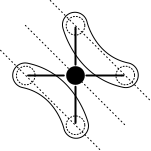
\includegraphics{grad_scatter_stencil}
  \caption{Stencil of the scatter-type algorithm}
  \label{fig:grad_scatter_stencil}
\end{figure}

\subsubsection{How I have implemented it}
As my implementation of the shape extension \(\mathfrak{K}_{ext}\) only contains
nodes that are required by equation \eqref{eq:shape_extension_requirement},
there is no necessity to use the scatter type strategy.
Instead my implementation uses the \emph{gather-type algorithm}. It loops over all
\(\mindex{k} \in \mathfrak{K}_{ext}\), gathers the values of its contributors
and finally computes the new coefficients \(c'_{\mindex{k}}\) according to equation
\eqref{eq:compute_grad_coeff}.
I decided to use this strategy, because it is much easier to parallelise than the
scatter-type algorithm.
For each node, the program just writes to one instead to \(2D\) locations.
This greatly simplifies parallelisation.

\begin{figure}[H]
  \centering
  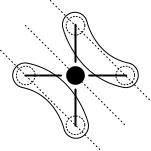
\includegraphics{grad_gather_stencil}
  \caption{Stencil of the gather-type algorithm.}
  \label{fig:grad_gather_stencil}
\end{figure}

\begin{algorithm}[H]
  \Input{Wavepacket dimension \(D\)}
  \Input{Scaling parameter \(\varepsilon\)}
  \Input{Wavepacket parameters \(\Pi=(\vec{q},\vec{p},\mat{Q},\mat{P},S)\)}
  \Input{Basis shape \(\mathfrak{K}\)}
  \Input{Basis shape extension \(\mathfrak{K}_{ext}\)}
  \Input{Wavepacket coefficients \(\boldsymbol{c} \in \mathbb{C}^{N \times 1}\) (array of scalars)}
  \Output{Coefficients of wavepacket gradient \(\boldsymbol{\vec{c'}} \in \mathbb{C}^{N \times D}\) (array of vectors)}
  \For{\(\mindex{k} \in \mathfrak{K}_{ext} \)}{
    \emph{Compute contribution of centre node}\;
    \(m \leftarrow 0 \in \mathbb{C}\)\;
    \If{\(\mindex{k} \in \mathfrak{K}\)}{
      \(m \leftarrow c_{\mindex{k}}\)\;
    }

    \emph{Compute contribution of backward neighbours}\;
    \(\vec{b} \leftarrow 0 \in \mathbb{C}^D\)\;
    \For{\(d \in \{1,\ldots,D\}\)}{
      \If{\(\mindex{k}-\mindex{e}^d \in \mathfrak{K}\)}{
        \(b_d \leftarrow \sqrt{k_d}c_{\mindex{k}-\mindex{e}^d}\)\;
      }
    }

    \emph{Compute contribution of forward neighbours}\;
    \(\vec{f} \leftarrow 0 \in \mathbb{C}^D\)\;
    \For{\(d \in \{1,\ldots,D\}\)}{
      \If{\(\mindex{k}+\mindex{e}^d \in \mathfrak{K}\)}{
        \(f_d \leftarrow \sqrt{k_d+1}c_{\mindex{k}+\mindex{e}^d}\)\;
      }
    }

    \emph{Merge contributions of every node to get the coefficients of the gradient}\;
    \(\vec{c'_k} \leftarrow m\vec{p}+\frac{\varepsilon}{\sqrt{2}}(\mat{\overline{P}}\vec{f}+\mat{P}\vec{b})\)
  }
  \caption{Computes coefficients of the wavepacket gradient \(-i\varepsilon^2\nabla \Phi\)}
\end{algorithm}

\section{Performance}

\subsection{Wavepacket evaluation}

I benchmarked the wavepacket evaluation and gradient construction
on the
Euler cluster\footnote{Measurements done in year 2015, the CPU is Intel Xeon E5-2697v2 (2.7 GHz).}
\cite{euler_cluster} using one thread.
I used a hyperbolic cut shape with limits \(10\), and varied the
sparsity between \(2^D\) and \(3^D\) to obtain different numbers of
basis functions for a given dimensionality \(D\).

\begin{figure}[H]
  \centering
  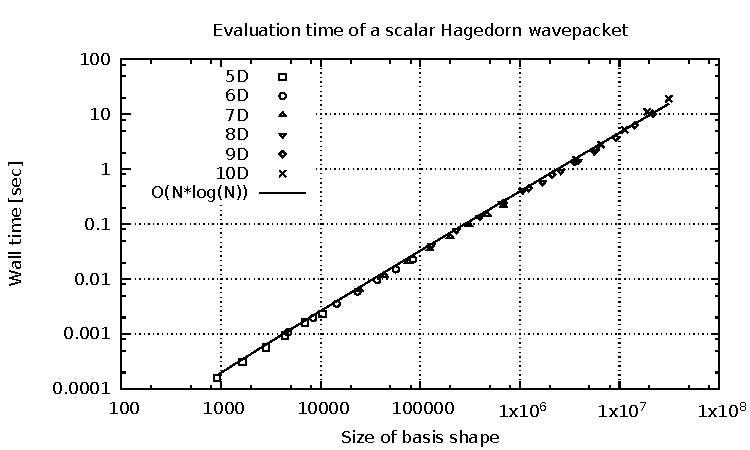
\includegraphics[width=1.0\textwidth]{plots/hawp_eval_runtime}
  \caption{Time to evaluate a scalar wavepacket on one node \(\vec{x}\).}
  \label{fig:hawp_eval_runtime}
\end{figure}

The plot (\ref{fig:hawp_eval_runtime}) shows that
evaluating a Hagedorn wavepacket with one million basis functions
on one grid node \(\vec{x}\) took 150 milliseconds.

Evaluating a Hagedorn wavepacket has an asymptotic run-time
complexity\footnote{Assuming \(\mathcal{O}(D) \approx \mathcal{O}(\log{}N)\).
See section (\ref{sec:hawp_eval_runtime_complexity}) for details.}
\(\mathcal{O}(N \log{}^2N)\)
where \(N\) is number of basis shape nodes. The measurements of runtime suggest \(\Theta(N\log{}N)\),
which is better because asymptotic limit has not been reached yet.

\begin{figure}[H]
  \centering
  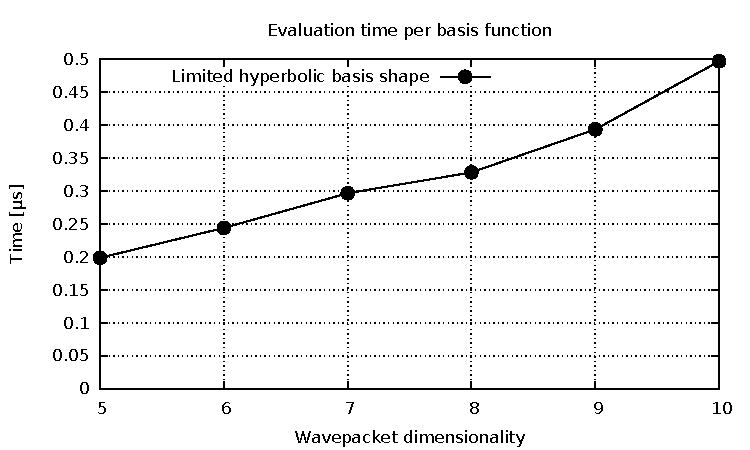
\includegraphics[width=1.0\textwidth]{plots/hawp_eval_efficiency}
  \caption{
    This chart shows the effect of dimensionality to evaluation time.
    It shows the time needed to evaluate \emph{one} basis function on one
    node \(\vec{x}\) depending on dimensionality.
  }
  \label{fig:hawp_eval_efficiency}
\end{figure}

\subsection{Gradient Computation}

Measurements reveal that gradient construction, i.e. computing the coefficients
of the gradient wavepacket, takes approximately six times longer than wavepacket evaluation.
Evaluating the gradient on one grid node \(\vec{x}\) takes \(2.5\) times longer.
That means, if the evaluation of some wavepacket \(\Phi_0\) takes \(1 ms\) time, than
computing the coefficients of the gradient wavepacket \(-i\varepsilon^2\nabla\Phi_0\) takes \(6ms\) time.
Evaluating the gradient \((-i\varepsilon^2\nabla \Phi_0)(\vec{x})\) on one node requires \(2.5 ms\) time.

\begin{figure}[H]
  \centering
  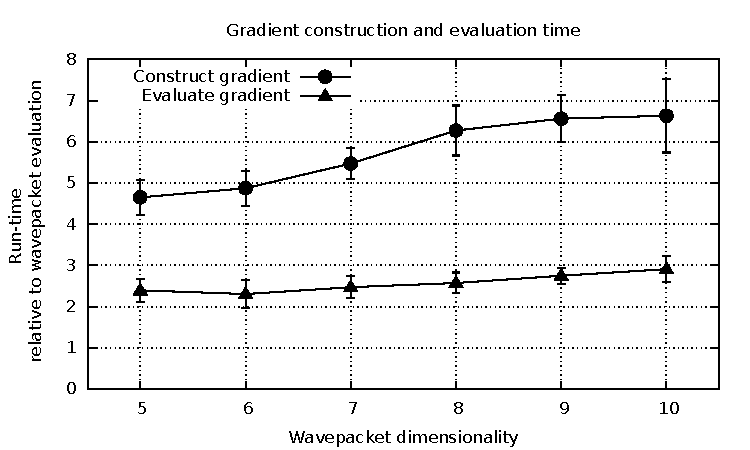
\includegraphics[width=1.0\textwidth]{plots/grad_reltime}
  \label{fig:grad_reltime}
  \caption{
    This plot shows two series: One depicts the time to construct a wavepacket gradient.
    The other depicts the time to evaluate a wavepacket gradient.
    Time is shown \emph{relative} to wavepacket evaluating.
    Error bars depict the standard deviation.
  }
\end{figure}

\subsection{Comparison to WaveBlocksND}

\subsubsection{Wavepacket evaluation}

\begin{figure}[H]
  \centering
  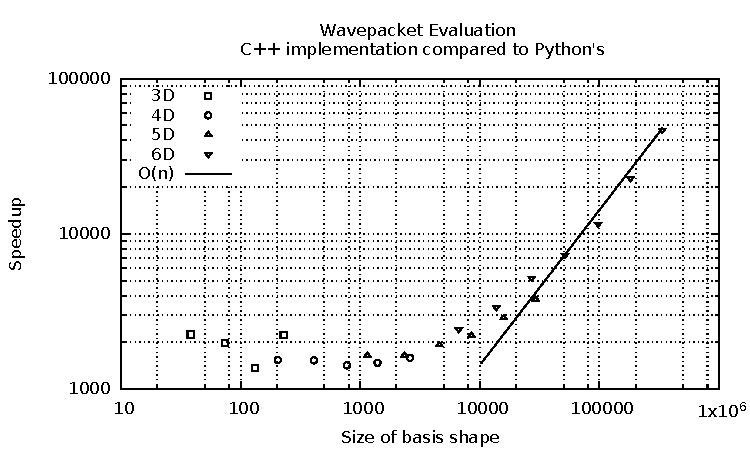
\includegraphics[width=1.0\textwidth]{plots/hawp_eval_cvp_slim}
  \caption{Wavepacket evaluation time in C++ compared to WaveBlocksND.
    WaveBlocksND uses the \textbf{slim recursion} routine.}
  \label{fig:hawp_eval_cvp_slim}
\end{figure}

Apparently, the C++ implementation is asymptotically better than
WaveBlocksND's slim recursion by a factor of \(\mathcal{O}(N)\).
My implementation could have slightly better run-time complexity due to slicing, but by
no means \(\mathcal{O}(N)\). The run-time complexity of the slim recursion is
quadratic to the basis shape size.
This behaviour is caused by a flaw, somewhere inside the slim recursion.
Due to this discovery, I've done all further comparisons using the fat recursion routine,
which behaves well, as seen in the figure below. On average, my implementation evaluates a
Hagedorn wavepacket 2000 times faster than WaveBlocksND.

\begin{figure}[H]
  \centering
  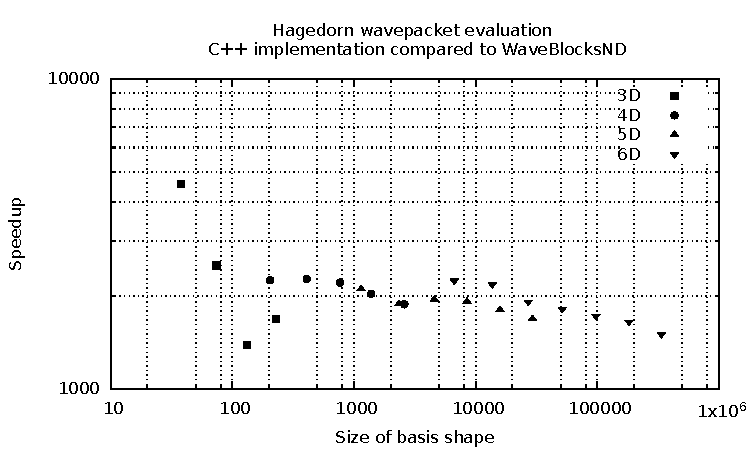
\includegraphics[width=1.0\textwidth]{plots/hawp_eval_cvp_fat}
  \caption{Wavepacket evaluation time in C++ compared to WaveBlocksND.
  WaveBlocksND uses the \textbf{fat recursion} routine.}
  \label{fig:hawp_eval_cvp_fat}
\end{figure}

\subsubsection{Gradient computation}

Below is a benchmark of the gradient computation. The employed wavepacket
has a limited hyperbolic cut basis shape\footnote{
  The cut-off limit is 100, sparsity varies between \(2^D\) and \(3^D\).}.
The results reveal run-time complexity improvements of my implementation.

\begin{figure}[H]
  \centering
  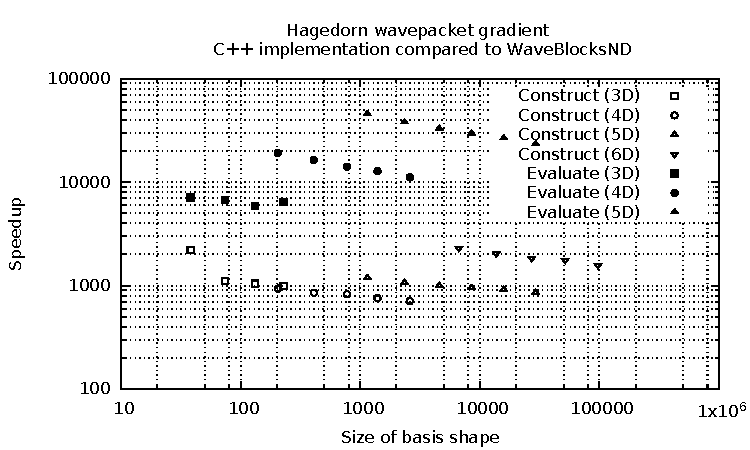
\includegraphics[width=1.0\textwidth]{plots/grad_eval_cvp}
  \caption{
    Wavepacket gradient construction and evaluation time in C++ compared to WaveBlocksND.
    Speedup means the run-time of WaveBlocksND divided by the run-time of my implementation.
    This chart contains two series: Empty bullets show the speedup when constructing
    the wavepacket gradient. Filled bullets show the speedup when evaluating the
    wavepacket gradient.
  }
  \label{fig:grad_eval_cvp}
\end{figure}

I've changed the way how shape extensions are generated. WaveBlocksND generates
shape extensions that contain many superfluous nodes. The ratio of superfluous to
essential nodes grows exponentially with the shape
dimensionality.\footnote{This effect is very apparent when using hyperbolic cut shapes.}
This results in a wavepacket gradient that has \(\mathcal{O}(\exp{}(D) N)\) basis functions instead of
\(\mathcal{O}(N)\).

WaveBlocksND mitigates this issue by constructing gradients using the scatter-type algorithm,
since the scatter-type algorithm simply ignores superfluous nodes. This works well for low dimension.
Nevertheless, the cost of allocating and zero-initialize oversized arrays
becomes apparent from dimensionality six.

My implementation generates shape extensions that only contain essential no\-des.
The \emph{evaluate}-series reflect the advantage of such tight shape extensions
when evaluating wavepacket gradients.

\subsection{First steps towards parallelisation using OpenMP}

I paid attention to possible parallelisation right from the start.
The evaluation of Hagedorn wavepackets is of quite serial nature, due to its
recursive scheme. But basis functions on the same slice can be evaluated independently.
This was one of my main reasons to split basis shapes into slices.
I added a simple \emph{pragma omp parallel for} to the loop, that runs over all nodes
of the same slice. I've done some measurements on the Euler cluster, using up to 12 threads.
The plot below (\ref{fig:hawp_eval_omp}) shows, that the evaluation of large and high dimensional
wavepackets scales reasonably well.

\begin{figure}[H]
  \centering
  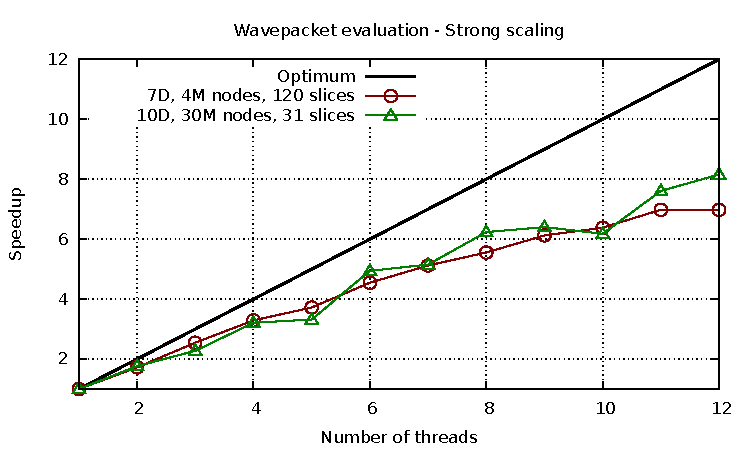
\includegraphics[width=1.0\textwidth]{plots/hawp_eval_omp}
  \caption{
    Strong scaling plot of the Hagedorn wavepacket evaluation.
    It shows two measurements: One of a 7-dimensional wavepacket with
    four million basis functions, the other of a 10-dimensional wavepacket with
    30 million basis functions.
  }
  \label{fig:hawp_eval_omp}
\end{figure}

\begin{figure}[H]
  \centering
  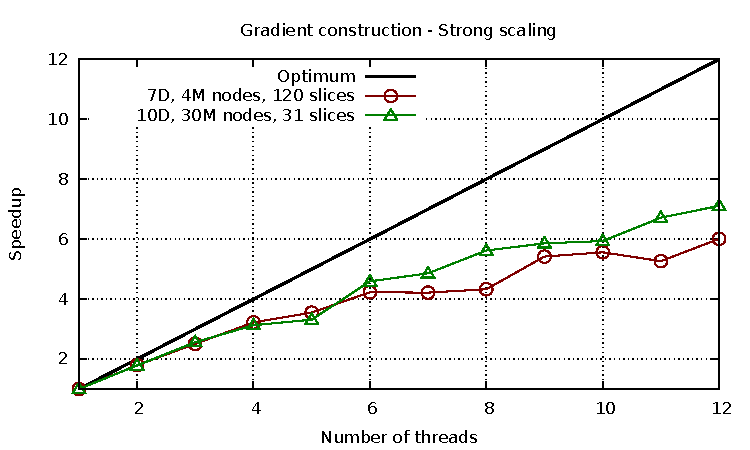
\includegraphics[width=1.0\textwidth]{plots/grad_eval_omp}
  \caption{
    Strong scaling plot of the wavepacket gradient construction.
    It shows two measurements: One of a 7-dimensional wavepacket with
    four million basis functions, the other of a 10-dimensional wavepacket with
    30 million basis functions.
  }
  \label{fig:grad_eval_omp}
\end{figure}

\bibliographystyle{plain}
\bibliography{references,../../references/own}

\end{document}

%%% Local Variables:
%%% mode: latex
%%% TeX-master: t
%%% End:
